% document type
\documentclass[12pt]{article}

% packages
\usepackage[total={170mm,230mm}]{geometry}
\usepackage[utf8]{inputenc}
\usepackage[T1]{fontenc}
\usepackage[russian]{babel}
\usepackage{graphicx}
\usepackage{amssymb}
\usepackage{amsfonts}
\usepackage{amsmath}
\usepackage{amsthm}
\usepackage{physics}
\usepackage{nicefrac}
\usepackage{cancel}
\usepackage{hyperref}
\usepackage{cmap}

\title{Дифракция Фраунгофера}
\author{Козлов Александр \and Краснощёкова Дарья}

\begin{document}
	\maketitle
	\section{Формулы для интенсивности дифракционной картины}
	Выведем из принципа Гюйгенса\---Френеля формулу для интенсивности в зависимости от угла дифракции. Пускай на решётку с периодом $d$ и щелями ширины $b$ падает свет амплитуды $E_0$ с длиной волны $\lambda$. Каждую щель разобьём на бесконечно малые излучатели ширины $\dd x$. Разность хода для излучателя с координатой $x$ и для излучателя с координатой $x=0$ будет
	\begin{equation}
		\Delta = x \sin{\theta}.
	\end{equation}
	Что следует из элементарных геометрических соображений (см. рис. \ref{fig:figure1}).
	\begin{figure}[htbp]
		\centering
		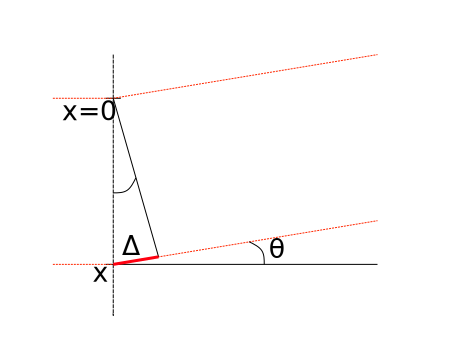
\includegraphics[width=\linewidth]{../images/fig1}
		\caption{Иллюстрация к вычислению разности хода.}
		\label{fig:figure1}
	\end{figure}
	Тогда комплексная амплитуда бесконечно малого излучателя с координатой $x$ испытает относительно комплексной амплитуды бесконечно малого излучателя с координатой $x=0$ сдвиг по фазе на $k\cdot\Delta$, где через $k$ обозначено волновое число. Комплексная амплитуда бесконечно малого излучателя с координатой $x$ будет
	\begin{equation}
	 	\dd \tilde{E}(x) = \dfrac{E_0}{b}\, e^{i k x \sin{\theta}}\dd x.
	\end{equation}
	Интегрируя по всей ширине щели, получаем зависимость комплексной амплитуды одной щели от $\sin{\theta}$
	\begin{equation}
		\tilde{E}_1\qty(\sin{\theta}) = E_0\, e^{i\dfrac{kb\sin{\theta}}{2}} sinc\qty(\dfrac{kb\sin{\theta}}{2}).
	\end{equation}
	Откуда сразу получаем формулу для интенсивности света для одной щели
	\begin{equation}
		I_1 = \tilde{E}_1 \qty(\tilde{E}_1)^* = I_0\, sinc^2\qty(\dfrac{kb\sin{\theta}}{2}).
	\end{equation}
	Что и требовалось проверить. 
	\par Рассмотрим случай $N$ щелей. Для $m$\--ой щели имеем (добавиться набег фазы)
	\begin{equation}
		\tilde{E}_m\qty(\sin{\theta}) = \tilde{E}_1\qty(\sin{\theta}) e^{ik(m-1)d\sin{\theta}}.
	\end{equation}
	Чтобы получить суммарную амплитуду, нужно просуммировать амплитуды всех щелей. Вычисляем сумму геометрической прогрессии
	\begin{equation}
	\begin{split}
		\tilde{E} =& \tilde{E}_1\qty(\sin{\theta})\, e^{-ikd\sin{\theta}}\, \sum_{m=1}^{N} e^{ikmd\sin{\theta}}\\
		=&\tilde{E}_1\qty(\sin{\theta})\, e^{-ikd\sin{\theta}}\, \dfrac{e^{ikd\sin{\theta}}\qty(1 - e^{ikdN\sin{\theta}})}{1-e^{ikd\sin{\theta}}}\\
		=&\tilde{E}_1\qty(\sin{\theta})\, e^{i\cdot (...)}\, \dfrac{\sin\qty(\dfrac{kdN\sin{\theta}}{2})}{\sin\qty(\dfrac{kd\sin{\theta}}{2})}.
	\end{split}
	\end{equation}
	Отсюда и получаем итоговую формулу для интенсивности дифракционной решётки из $N$ щелей
	\begin{equation}
		I_N =  I_0\, sinc^2\qty(\dfrac{kb\sin{\theta}}{2})\, \dfrac{\sin^2\qty(\dfrac{kdN\sin{\theta}}{2})}{\sin^2\qty(\dfrac{kd\sin{\theta}}{2})}.
	\end{equation}

	\section{Наблюдение дифракционной картины для различных решёток}
	\subsection{Дифракция на одной щели}


	\section{Сравнение результатов наблюдений с теорией}

	\section{Качественный наблюдения}
\end{document}